\begin{figure}[H]
  \centering
  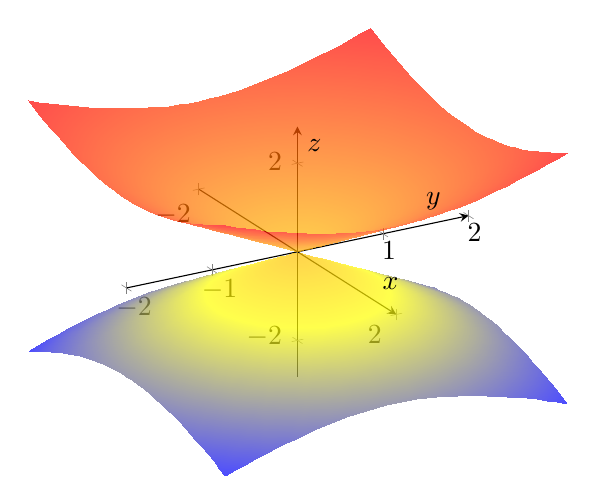
\begin{tikzpicture}
    \begin{axis}[
      view={60}{30},
      axis lines=middle,
      xlabel={$x$},
      ylabel={$y$},
      zlabel={$z$},
      domain=-2:2,
      y domain=-2:2,
      samples=35,
      mesh/ordering=y varies,
      z buffer=sort,
      grid=major,
    ]

    % Folha superior: z = +sqrt(x^2 + y^2)
    \addplot3[
      surf,
      shader=interp,
      opacity=0.7
    ]
    {sqrt(x^2 + y^2)};

    % Folha inferior: z = -sqrt(x^2 + y^2)
    \addplot3[
      surf,
      shader=interp,
      opacity=0.7
    ]
    {-sqrt(x^2 + y^2)};

    \end{axis}
  \end{tikzpicture}
\end{figure}
